%%%%%%%%%%%%%%%%%%%%%%% file template.tex %%%%%%%%%%%%%%%%%%%%%%%%%
%
% This is a general template file for the LaTeX package SVJour3
% for Springer journals.          Springer Heidelberg 2010/09/16
%
% Copy it to a new file with a new name and use it as the basis
% for your article. Delete % signs as needed.
%
% This template includes a few options for different layouts and
% content for various journals. Please consult a previous issue of
% your journal as needed.
%
%%%%%%%%%%%%%%%%%%%%%%%%%%%%%%%%%%%%%%%%%%%%%%%%%%%%%%%%%%%%%%%%%%%
%
\RequirePackage{fix-cm}
%
%\documentclass{svjour3}                     % onecolumn (standard format)
\documentclass[smallcondensed]{svjour3}     % onecolumn (ditto)
%\documentclass[smallextended]{svjour3}      % onecolumn (second format)
%\documentclass[twocolumn]{svjour3}          % twocolumn
%
\smartqed  % flush right qed marks, e.g. at end of proof
%
\usepackage{graphicx}
%
% \usepackage{mathptmx}      % use Times fonts if available on your TeX system
%
% insert here the call for the packages your document requires
%\usepackage{latexsym}
% etc.
%
% please place your own definitions here and don't use \def but
% \newcommand{}{}
%
% Insert the name of "your journal" with
\journalname{AStA Advances in Statistical Analysis}

% Own Packages and newcommands
\usepackage{amsmath, amssymb}
\setlength{\parindent}{0pt} % remove indentation before every paragraph
\usepackage{booktabs}
\usepackage{multirow}
\usepackage{float} % to force figure placement
\usepackage[usenames, dvipsnames]{color}
% \usepackage[backend=bibtex,
%             style=nature,
%             citestyle=authoryear]{biblatex}
% \addbibresource{bauer_2018.bib}
\usepackage{natbib}
\bibliographystyle{smj}
\newcommand{\T}{\mathrm{\scriptscriptstyle T}}
\newcommand{\red}[1]{\textcolor{red}{#1}}



\begin{document}
\title{KOALA: Estimating coalition probabilities in multi-party electoral systems%\thanks{Grants or other notes
%about the article that should go on the front page should be
%placed here. General acknowledgments should be placed at the end of the article.}
}
\subtitle{Do you have a subtitle?\\ If so, write it here}
\titlerunning{KOALA: Coalition analyses}   % if too long for running head

\author{Alexander Bauer \and Andreas Bender \and Andr\'e Klima \and Helmut K\"{u}chenhoff}

%\authorrunning{Short form of author list} % if too long for running head

\institute{A. Bauer \at
              Statistical Consulting Unit StaBLab, Department of Statistics, LMU Munich, Germany \\
              Tel.: +49-89-2180-3197 \\
              Fax: +49-89-2180-5308 \\
              \email{alexander.bauer@stat.uni-muenchen.de} \\
              ORCID: 0000-0003-3495-5131
%             \emph{Present address:} of F. Author  %  if needed
           \and
           A. Bender \at
              Statistical Consulting Unit StaBLab, Department of Statistics, LMU Munich, Germany \\
              ORCID: 0000-0001-5628-8611
           \and
           A. Klima \at
              Statistical Consulting Unit StaBLab, Department of Statistics, LMU Munich, Germany
           \and
           H. K\"{u}chenhoff \at
              Statistical Consulting Unit StaBLab, Department of Statistics, LMU Munich, Germany
}

\date{Received: date / Accepted: date}
% The correct dates will be entered by the editor


\maketitle

\begin{abstract} \red{150 to 250 words} \\
Common election poll reporting is often misleading as sample uncertainty is either not covered at all or only insufficiently. For a more comprehensive coverage, we propose shifting the focus towards reporting survey-based probabilities for specific election outcomes. We present such an approach for multi-party electoral systems, focusing on probabilities of coalition majorities. A Monte Carlo based Bayesian Multinomial-Dirichlet model is used for estimation. The method utilizes published opinion polls
%conducted by established polling agencies
and is accompanied by a pooling approach to summarize multiple current surveys, accounting for dependencies between polling agencies.
%Potential biases of specific pollsters are not taken into account.
Sample uncertainty-based probabilities are estimated, assuming the election was held today. An implementation in \texttt{R} is freely available.

\keywords{\red{4 to 6 keywords} Election analysis \and Opinion polls \and Election reporting \and Multinomial-Dirichlet \and Pooling}
% \PACS{PACS code1 \and PACS code2 \and more}
% \subclass{MSC code1 \and MSC code2 \and more}
\end{abstract}

\section{Introduction and data} \label{intro}
Election polls
%are conducted by different polling agencies and
try to represent the public opinion based on a finite sample.
Usually, polling agencies publish the shares of the electorate
who would vote for the reported political parties {\it if the election was held today},
the number of overall respondents and -- more or less prominent -- information
about the uncertainty of the results.
Current reporting of general media on such surveys in the end is most
often limited to the observed shares, while sample uncertainty
is usually ignored or only covered insufficiently.

Prominent examples for inaccurate reporting can be found
in multi-party electoral systems.
In such, one party usually doesn't obtain enough votes for a majority.
In these situations, multiple parties form a so-called coalition
to jointly obtain the necessary majority share of seats in parliament.
Often then, a coalition is stated to ``lose'' its majority
just because the joint poll share drops under 50\% from one opinion poll to
the next \citep[cf.][]{umfrage_2017}.
Such interpretations are clearly misleading as opinion polls are based on a finite sample
of voters and only allow conclusions about the whole electorate
with a specific certainty. Reporting results in this manner thus
reinforces general misunderstandings of the public about which message
to draw from published opinion polls. Additionally, the perception of
the observed voter shares to be definite values that hold for the
electorate can also lead to an -- to some extent -- unjustified criticism
of general opinion polls if the final election result differs
from the latest polls published before election day. One prominent example is
\red{XXX hier wenn moeglich a Beispiel fuer so a unberechtigte Kritik an Umfragen nach da Wahl XXX} (QUELLE).

Beyond ensuring proper reporting of sample uncertainties, in our opinion, the
whole focus in survey reporting should be shifted from describing the raw
observed party shares. Instead, reporting should focus on the most relevant
question, i.e. {\it how probable} specific events or election outcomes are.
Events of interest can range from probabilities for parties passing
a specific voter share via one party obtaining more seats in parliament
than another through to probabilities for majorities of potential multi-party coalitions.
As such probabilities combine both -- the observed raw voter share
and sample uncertainty -- in one number, they are in theory easier to
communicate to the general public. \red{Evtl (hier oder in da Discussion) auf de geplante Graefe-Studie verweisen, der de Vermittelbarkeit vo soichane W'keiten untersuacha mecht.}

We present our KOALA (Coalition Analysis) approach to estimate such probabilities
to bring more value to opinion poll-based reporting, specifically focusing on
multi-party electoral systems and the estimation of probabilities for coalition
majorities. To estimate the probabilities, a Bayesian Multinomial-Dirichlet model
with Monte Carlo simulations is used. Also, a pooling approach is presented to summarize
multiple current opinion polls to reduce sample uncertainty.
Prior to the German federal elections 2013 and 2017, results based on (an earlier iteration of)
our approach already entered general media reporting \citep[cf.][]{wahlistik_2013, gelitz_2017}.

As database, we use opinion polls conducted by established polling agencies,
quantifying the electoral behavior \textit{if an election was held today}.
We focus on the question of quantifying current majority situations, not
taking into consideration potential shifts until election day.
Approaches for predicting future election outcomes based on past
information can e.g. be found in \citet{graefe_2017} or \citet{norpoth_gschwend_2010}.

All methods were implemented in \texttt{R} \citep{r_2017} and are available in the open-source
package \texttt{coalitions} on GitHub \citep{bender_bauer_2018}. An
interactive \texttt{shiny}-based \citep{chang_2017} website \texttt{koala.stat.uni-\allowbreak muenchen.\allowbreak de}
visualizes estimated coalition probabilities and is used to communicate the results to the general public, covering German federal and state-wide elections.
The process of fetching new polls, updating the website and sending out Twitter messages based on the newest results is automated and allows for an immediate transfer of the estimated event probabilities to media and pulic.



\section{Calculation of probabilities} \label{sec:method}
In the last opinion poll conducted before the German federal election 2013 \citep{forsa_2013}, special interest was on whether CDU/CSU-FDP (also ``Union-FDP'') would obtain enough votes to form the governing coalition:

\begin{table}[!ht]\centering
\caption{Observed voter shares in the Forsa opinion poll for the German federal election, published September 20th, 2013 with $n=1995$ respondents
\label{bauer:tab_fdp}
}
\medskip
\begin{tabular}{cccccccc}
\toprule[0.09 em]
Union & SPD & Greens & FDP & The Left & Pirates & AfD & Others \\
\midrule
40\% & 26\% & 10\% & 5\% & 9\% & 2\% & 4\% & 4\% \\
\bottomrule[0.09 em]
\end{tabular}
\end{table}

The German election system mandates a 5\% votes share for parties to enter the parliament.
Votes for parties below this threshold are redistributed (proportionally) to parties
above it, leading to the following redistributed party shares:

\begin{table}[!ht]\centering
\caption{Redistributed party shares based on the Forsa opinion poll for the German federal election, published September 20th, 2013 with $n=1995$ respondents. Parties marked with ''--'' didn't pass the 5\% hurdle.
\label{bauer:tab_fdp_redist}
}
\medskip
\begin{tabular}{cccccccc}
\toprule[0.09 em]
Union & SPD & Greens & FDP & The Left & Pirates & AfD & Others \\
\midrule
44.44\% & 28.89\% & 11.11\% & 5.56\% & 10.00\% & -- & -- & -- \\
\bottomrule[0.09 em]
\end{tabular}
\end{table}

As can be seen in Table \ref{bauer:tab_fdp_redist}, Union-FDP with its 45\% raw voter share would get exactly 50\% of parliament seats after redistribution. Thus, ingoring uncertainty one would conclude that a majority of the coalition is slightly missed. However, it is clear that this only holds with a certain probability and particularly depends on whether FDP, Pirates and AfD each pass the 5\% hurdle.

The model to estimate event probabilities is based on the Multinomial distribution of the observed
number of voters per party. Therefore, we use a Bayesian Multinomial-Dirichlet model
with Jeffreys prior as an uninformative prior for the true party shares
$\theta_j$ \citep{gelman_2013}:
% \begin{equation}
% (\theta_1,\ldots,\theta_k)^\T \sim Dirichlet(\alpha_1,\ldots,\alpha_k), \ \ \text{with} \ \ \alpha_1 = \ldots = \alpha_k = \frac{1}{2}
% \end{equation}
\begin{equation}
\begin{aligned}
\boldmath{\theta} &= (\theta_1,\ldots,\theta_k)^\T \sim Dirichlet(\alpha_1,\ldots,\alpha_k), \\
\text{with} &\ \ \ \ \ \ \ \ \ \ \ \ \ \ \ \alpha_1 = \ldots = \alpha_k = \frac{1}{2}
\end{aligned}
\end{equation}
Given one (pooled) survey, the posterior in this case also is a Dirichlet distribution
with $\alpha_j = x_j + \frac{1}{2}$ for each party $j$ and its observed
vote counts $x_j$.

Using Monte Carlo simulations of election outcomes, one can obtain
specific event probabilities by taking their relative frequency of
occurence. E.g., if a specific event occurs in $2,600$ of $10\,000$
simulations this equals an estimated probability of $26\%$.

If an underrepresentation or overrepresentation of parties
in the polls of specific polling agencies is known, this information
can be included in the model by using an informative prior distribution,
where underrepresented parties would get higher $\alpha_j$ values and
overrrepresented parties would get lower $\alpha_j$ values, respectively.
However, such biases of polling agencies are hard to quantify
and we therefore use an ininformative prior.

Before applying the Bayesian approach and as vote shares are usually rounded
before publication, we adjust the available data by adding uniformly distributed
random noise to the
observed voter shares $x_j$ to avoid a potential bias caused by the use of
rounded numbers:
\begin{equation}
\begin{aligned}
x_{j,adj} = \ &x_j + r_{\gamma,j}, \\
\text{with} \ \ \ \ \ &r_{\gamma,j} \sim U[-\gamma,\gamma].
\end{aligned}
\end{equation}
E.g., for data rounded to $0.5\%$ we use a correction term of $\gamma = 0.5\%$. Afterwards, the adjusted shares are rescaled to ensure a sum of $100\%$ and the Bayesian approach is performed based on the adjusted shares.


\paragraph{Visualization} \ \\
Figure \ref{fig:seatDist} shows the simulated
parliament seat shares for the coalition Union-FDP, based on the observed
voter shares in Table \ref{bauer:tab_fdp}. The estimated density is clearly bimodal
as the observed FDP share before redistribution is exactly $50\%$ and
so FDP only enters the parliament in half of the simulations. The corresponding
probability for a seat majority of Union-FDP is $26.33\%$.

\begin{figure}[H]\centering
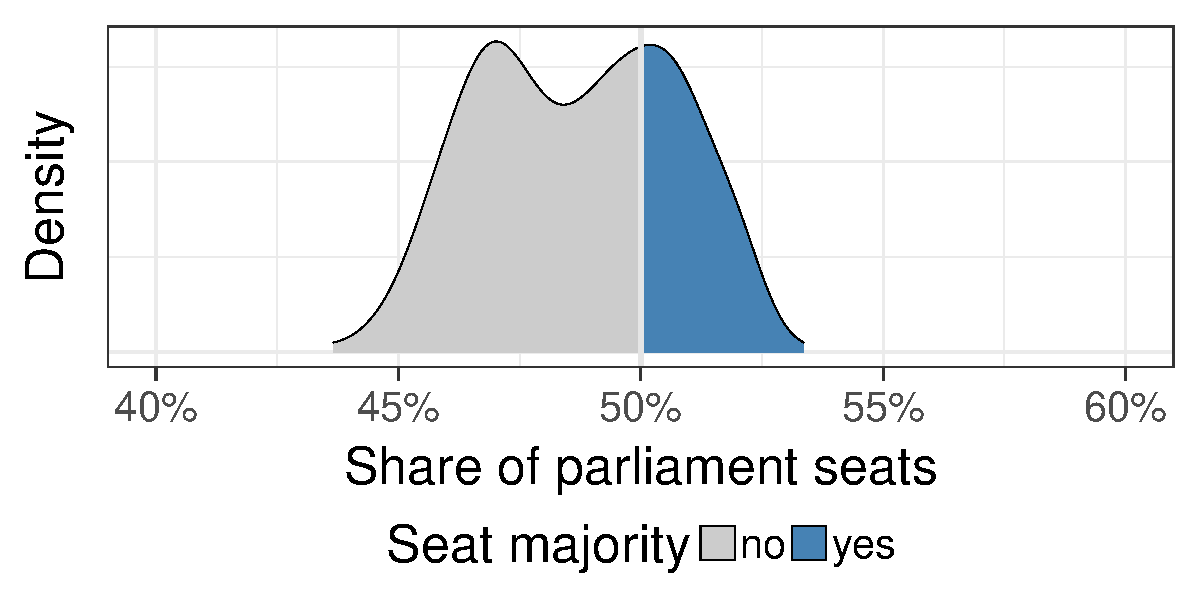
\includegraphics[width=0.35\textwidth]{figures/2013_forsa_cdufdp_lastPreelectionPoll.pdf}
\caption{Density of $10\,000$ simulated parliament seat shares for the coalition Union-FDP before the German federal election in September 2013 based on the Forsa opinion poll in Table \ref{tab_fdp}. The part of the density encoding for seat majorities is colored blue.
\label{fig:seatDist}
}
\end{figure}

As such density plots depict both the probability and the underlying
uncertainty for specific coalitions, they are a nice possibility to communicate
uncertainties underlying opinion polls to the general public. As the estimation
of event probabilities with our approach, such plots can be created for all
kinds of specific election outcomes.

\begin{figure}[H]\centering
\begin{tabular}{ll}
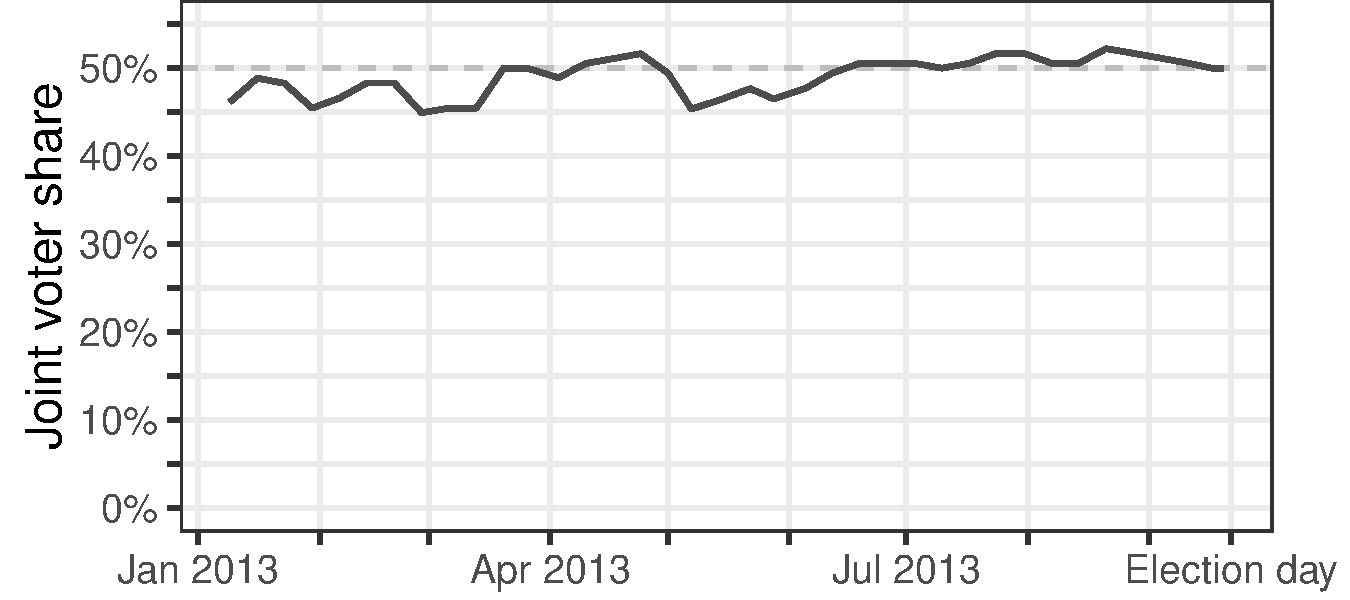
\includegraphics[height=.15\textwidth]{figures/2013_forsa_cdufdp_rawSharesRedist.pdf}
&
\multirow{2}{*}[13ex]{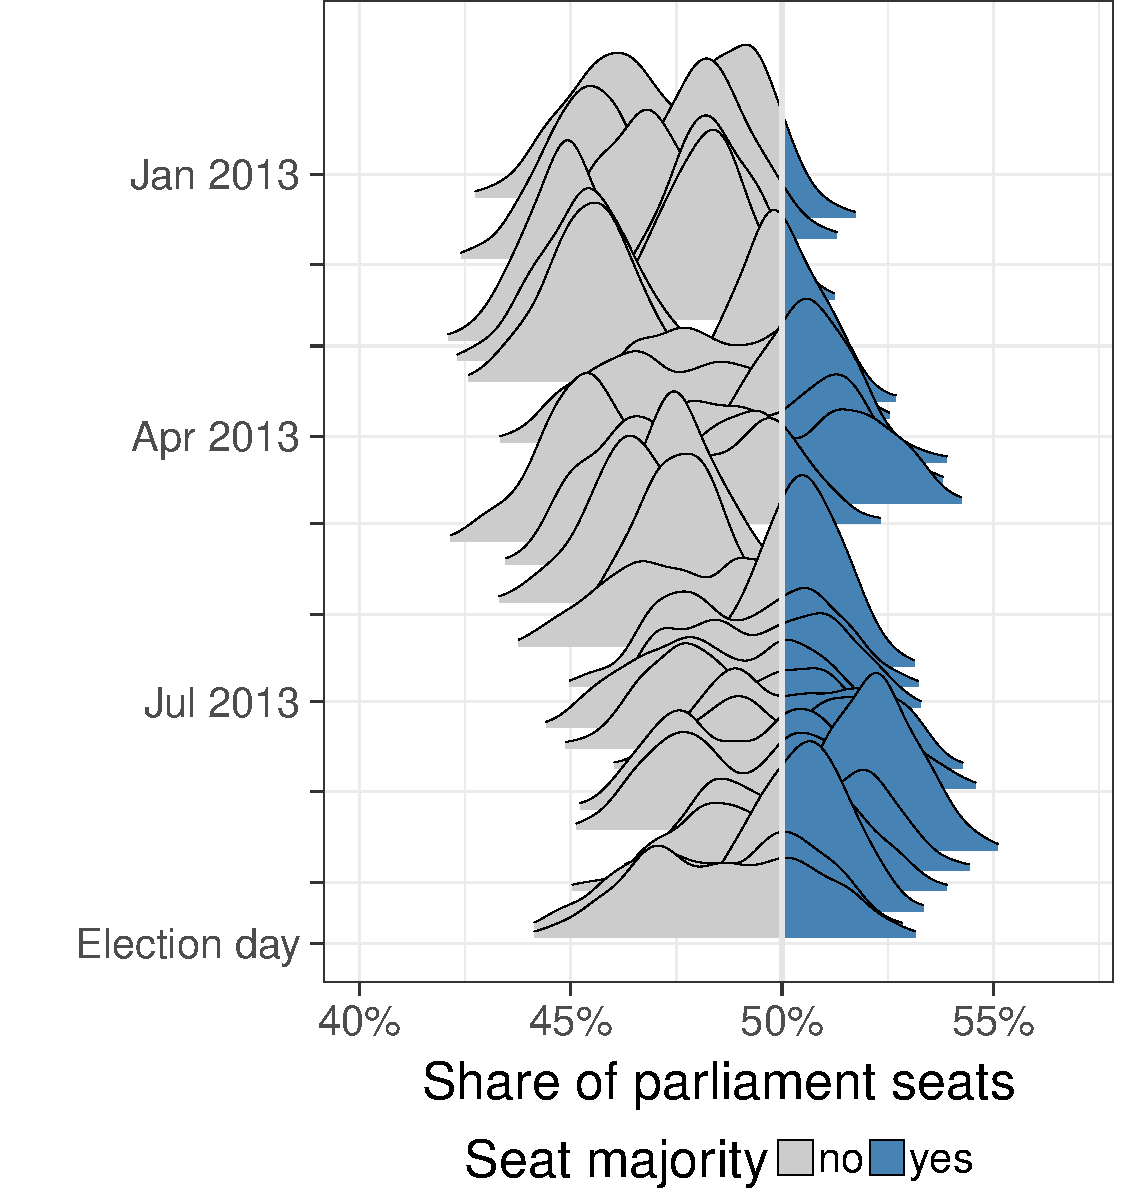
\includegraphics[height=30ex]{figures/2013_forsa_cdufdp_ridgeline.pdf}}
\\
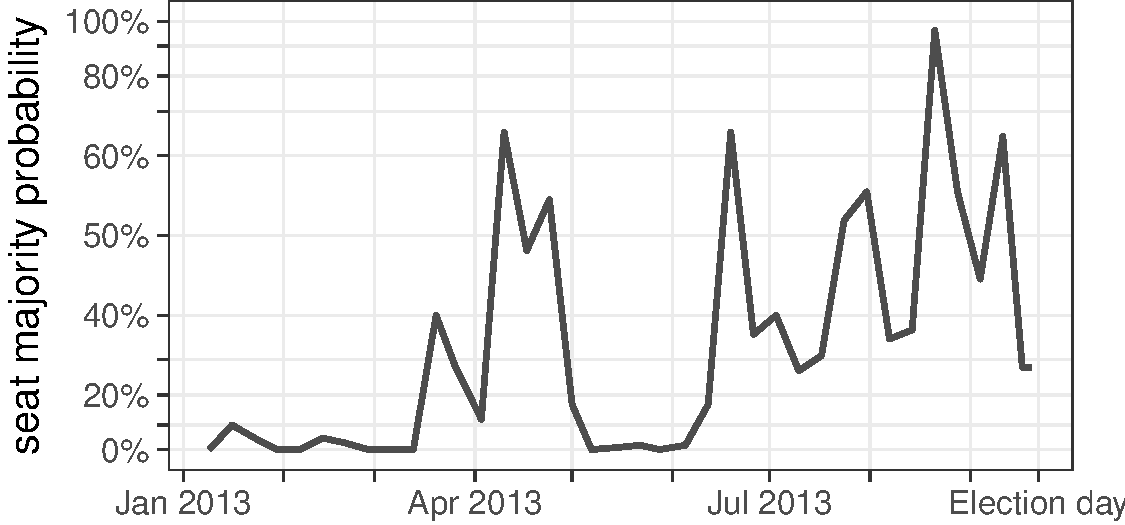
\includegraphics[height=.15\textwidth]{figures/2013_forsa_cdufdp_prob.pdf}
\end{tabular}
\caption{Development of the governing possibility of the coalition Union-FDP before the German federal election in September 2013 based on Forsa opinion polls.
Left top: Observed voter shares after redistribution. Left bottom: Probabilities to reach a majority of seats in parliament, based on $10\,000$ simulations. Right: Densities of simulated parliament seat shares based on $10\,000$ simulations. The parts of the densities encoding for seat majorities are colored blue.
\label{fig:seatDist_time}
}
\end{figure}

To visualize the {\it development} of such probabilities
%together with the underlying uncertainty
for a specific coalition we recommend extending the visualization of Figure \ref{fig:seatDist} by using ridgeline plots \citep{wilke_2017} for the simulated seat distributions. In Figure~\ref{fig:seatDist_time} this plot type and the development of majority probabilities is compared to
the raw, redistributed shares, which are usually reported in media.

Comparing the redistributed voter shares and the seat majority probabilities
in Figure~\ref{fig:seatDist_time} it is clear that the probabilities consist
of a lot more information than the voter shares. Especially, even small changes
in the redistributed voter shares can make an immense difference regarding the
chance of the coalition to form a government.

To focus on the most relevant changes in the majority probabilities, we propose
the use of a skewed axis as shown in Figure~\ref{fig:seatDist_time}. This axis
stretches the range of values around $50\%$ as a change in absolute probabilities
from $40\%$ to $60\%$ is more relevant than a change from $70\%$ to $90\%$ as
a success for achieving a seat majority is becoming more probable than a failure
to do so, or in both cases a success is already very probable, respectively.



\section{Pooling approach} \label{sec:pooling}
In the presence of multiple published opinion polls, pooling is used to
summarize the observed results in order to reduce sample uncertainty.
To assure a reliable pooling regarding the current public opinion,
we only use polls published within the past 14 days and only use the
most recent survey published by each polling agency.

Looking at a single poll $i$, the observed number of votes $X_{ij}$ for each of $k$ parties follow a multinomial distribution with sample size $n_i$ and underlying, unknown party shares $\theta_j$ in the population.
% \begin{equation}
% X_{i1},\ldots, X_{ik} \sim Multinomial(n_i,\theta_1,\ldots,\theta_k).
% \end{equation}
Pooling over multiple such polls as independent random samples leads to another multinomial distribution for the summed number of votes $\sum_i X_{ij}$:
% Based on the multinomial distribution of the vote counts $X_{ij}$ of party $j$ in poll $i$ with underlying true party share $\theta_j$, pooling over multiple polls representing independent random samples would lead to a multinomial distribution for the summed number of votes $\sum_i X_{ij}$:
\begin{equation}
\sum\limits_i X_{i1},\ldots, \sum\limits_i X_{ik} \sim Multinomial \left( \sum\limits_i n_i,\theta_1,\ldots,\theta_k \right).
\end{equation}

Further analyses, however, show that polls from different
polling agencies are correlated
and the independency assumption does not hold.
Therefore, we adjust the resulting multinomial
distribution by using an \textit{effective sample size} \citep{hanley_2003},
reflecting that the aggregation over multiple polls does not reflect the 
information from a sample with $\sum_i n_i$ observations.

Quantification of pairwise correlation is done based on the variance of the
difference between two polls. The following equation holds for two independent
random sample polls $A$ and $B$:

\begin{equation}
\begin{aligned}
Var(X_A - X_B) &= Var(X_A) + Var(X_B) - 2 \cdot Cov(X_A, X_B) \\
\Leftrightarrow \ \ \ \ Cov(X_{Aj}, X_{Bj}) &= \frac{1}{2} \cdot \left(Var(X_{Aj}) + Var(X_{Bj}) - Var(X_{Aj} - X_{Bj}) \right).
\end{aligned}
\end{equation}

We take $Var(X_{Aj})$ and $Var(X_{Bj})$ as the theoretical variances of the binomially distributed, observed voter numbers and estimate $Var(X_{Aj} - X_{Bj})$ based on the observed differences between the party shares. Having done so, one can estimate the covariance $Cov(X_{Aj}, X_{Bj})$ and accordingly also the correlation. As the binomial distribution is directly proportional to the sample size, the effective sample size $n_{\text{eff}}$ can be defined as the ratio between the estimated variance for the pooled sample and the theoretical variance of a sample of size one:
$$
n_{\text{eff}} = \frac{Var(\text{pooled})}{Var(\text{sample of size 1})},
$$
with, in the case of two surveys,
$$
Var(\text{pooled}) = Var(X_A + X_B) = Var(X_A) + Var(X_B) + 2 Cov(X_A,X_B)
$$
and $Var(\text{sample of size 1})$ the theoretical variance of the pooled share.

Looking at the party-specific correlations between 20 surveys conducted by the two most regular German polling agencies, Emnid and Forsa, we on average end up with a medium high correlation, using mean party shares and sample sizes per institute for the theoretical variances. Other institute comparisons were not performed as too few published surveys were conducted cover comparable time frames. For simplicity, we do not recalculate the correlation for each simulation, but rather set the correlation used in our methodology to $0.5$.
For convenience, the calculation of $n_{\text{eff}}$ is based on the party with most votes, as the specific party choice only marginally affects the results.

In the case of two published polls with $1500$ and $2000$ respondents, respectively, and a pooled share of $40\%$
for the strongest party, the method leads
to an effective sample size of $n_{eff} = 2341$. Thus, the method reduces sample uncertainty
compared to using only single polls, but the method is also clearly conservative, compared to
assuming independence between the polls and using a summed sample size of $1500 + 2000 = 3500$.

As noted, in practice we use a timeframe of 14 days, i.e. all surveys published at maximum 14 days ago are included
in the calculation of the pooled sample. In the case of opinion polls for a specific election getting published
only very rarely one can also extend this timeframe, e.g. using the heuristic of including all surveys published up to 14 days
ago with weight 1 (using their whole sample size), and all surveys within 14 to 28 days before today with halved weight
(using the halved sample size).



\section{Application} \label{sec:application}
We applied (an earlier iteration of) our method to the German federal elections
2013 and 2017, accompanied by news coverage in general media \citep[cf.][]{wahlistik_2013, gelitz_2017}.
In the following, we take these two elections as examples to underline
the differences between standard media reporting on opinion polls and our approach,
which focus on interpreting the raw observed shares after redistribution and
the estimated Bayesian probabilities, respectively.

For each election, 2013 and 2017, we base the event probabilities on
pooled surveys, which use the opinion polls published by the major
German polling agencies, i.e. Allensbach, Emnid, Forsa, Forschungsgruppe Wahlen,
GMS, Infratest dimap and INSA.
Opinion poll data from these polling agencies is publicly available1
on \texttt{www.wahlrecht.de}. 


\subsection{German federal election 2013} \label{subsec:2013}
From 2009 to 2013, the German government was formed by a coalition of 
conservative CDU/CSU (or ''Union'') and the liberal FDP. 
Thus, main interest before the election on September 22nd was in whether this
coalition could maintain its majority of parliament seats. As FDP in opinion
polls was very close to a voter share of $5\%$, i.e. the minimum hurdle to
pass into parliament, FDP successfully passing into parliament was crucial
for the success of the coalition.


\paragraph{Union-FDP coalition majority} \ \\
Figure \ref{fig:2013_cdufdp} visualizes the pooled opinion poll results
for the potential coalition Union-FDP, since one year before the election.
Starting from a redistributed voter share of around $43\%$ in October 2012,
the voter share in the pooled results rose steadily, reaching its maximum
of ca. $51\%$ about one month before election day.

Only taking this development of the redistributed voter share into
consideration, one would conclude that -- apart from a short
time window in August/September of 2013 -- a majority of the Union-FDP
coalition would not be possible if elections would have been held.
In the best case, sample uncertainty would be mentioned, making
a majority for the coalition {\it (highly) improbable}, but a more
solid quantification of uncertainty is not easily possible.

\begin{figure}[H]\centering
\begin{tabular}{ll}
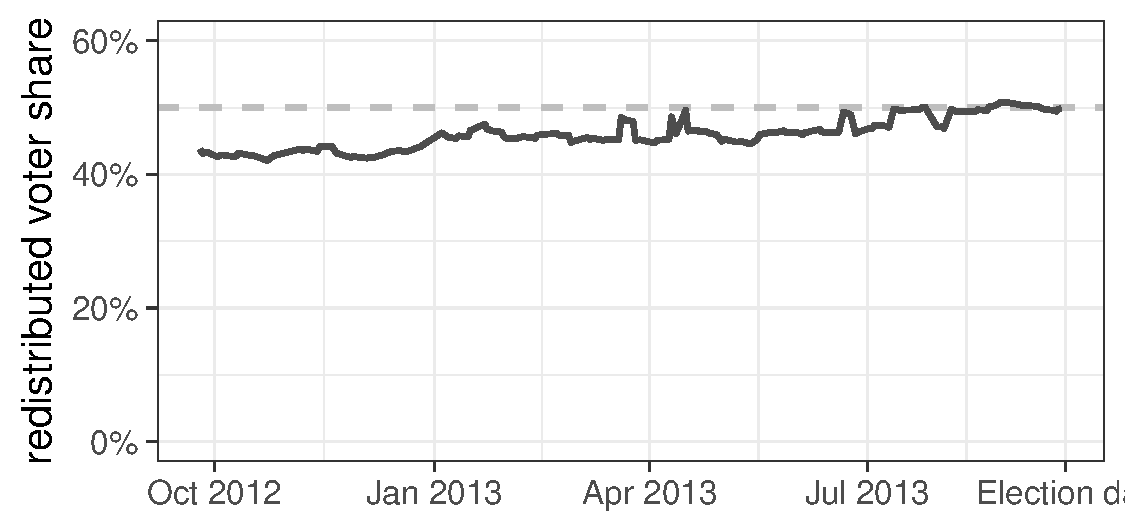
\includegraphics[height=.15\textwidth]{figures/2013_pooled_cdufdp_rawSharesRedist.pdf}
&
\multirow{2}{*}[13ex]{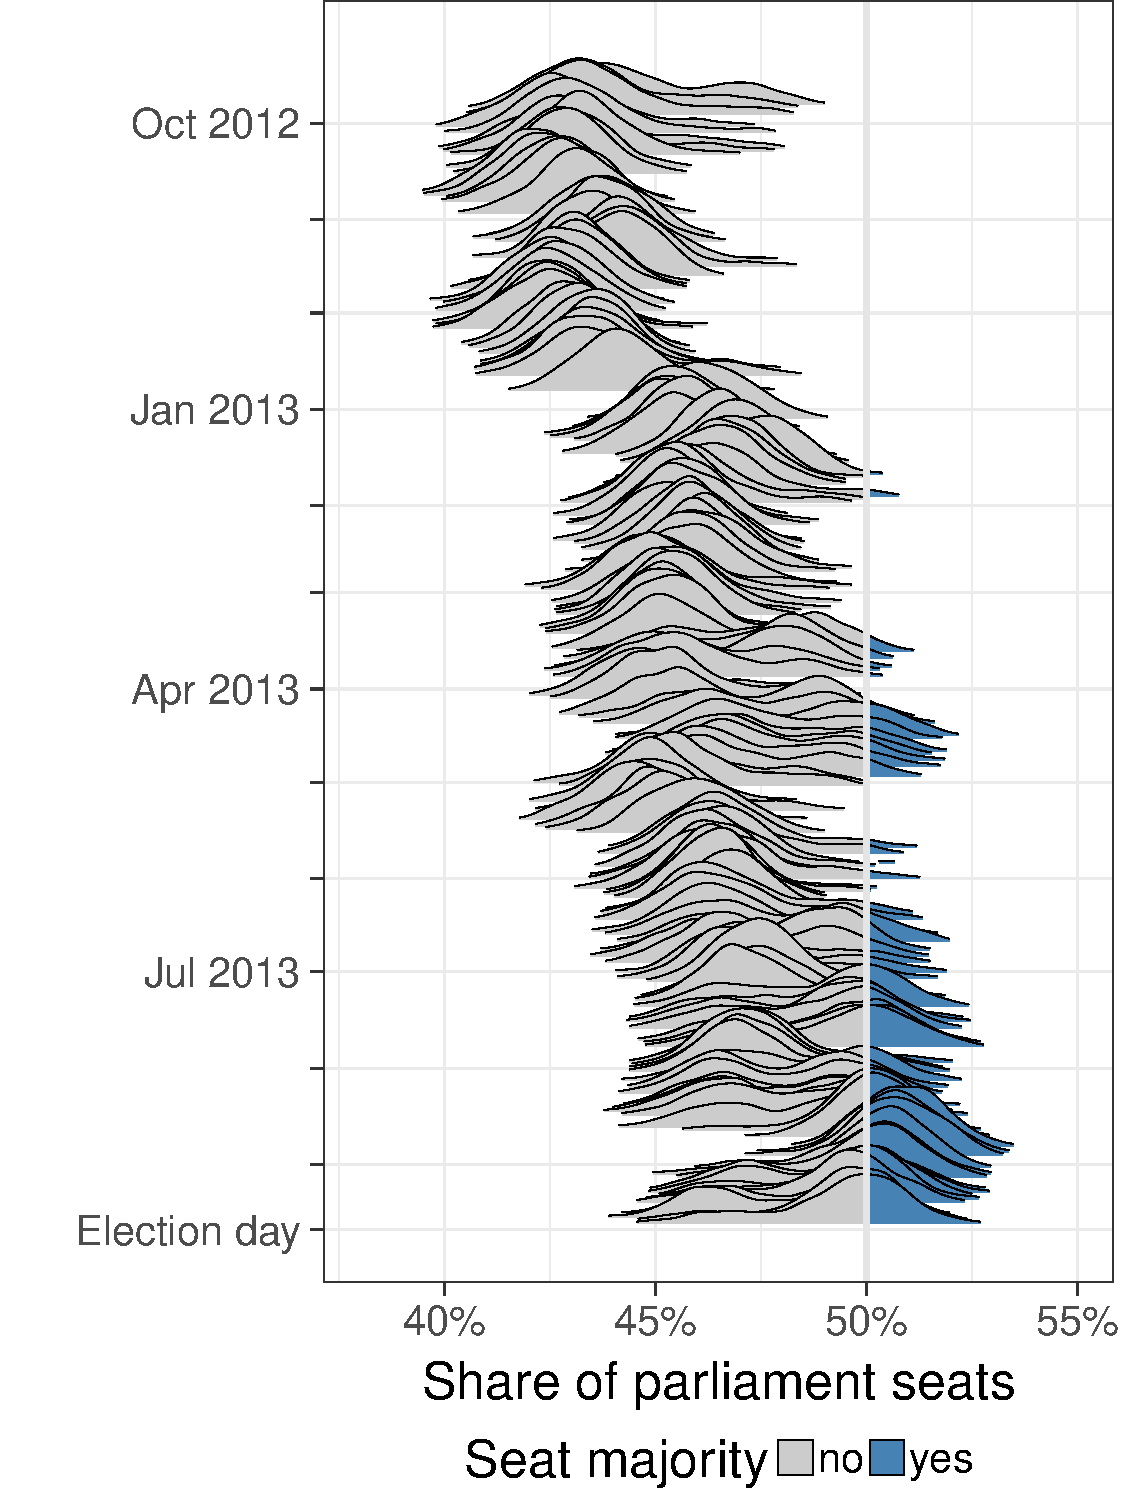
\includegraphics[height=30ex]{figures/2013_pooled_cdufdp_ridgeline.pdf}}
\\
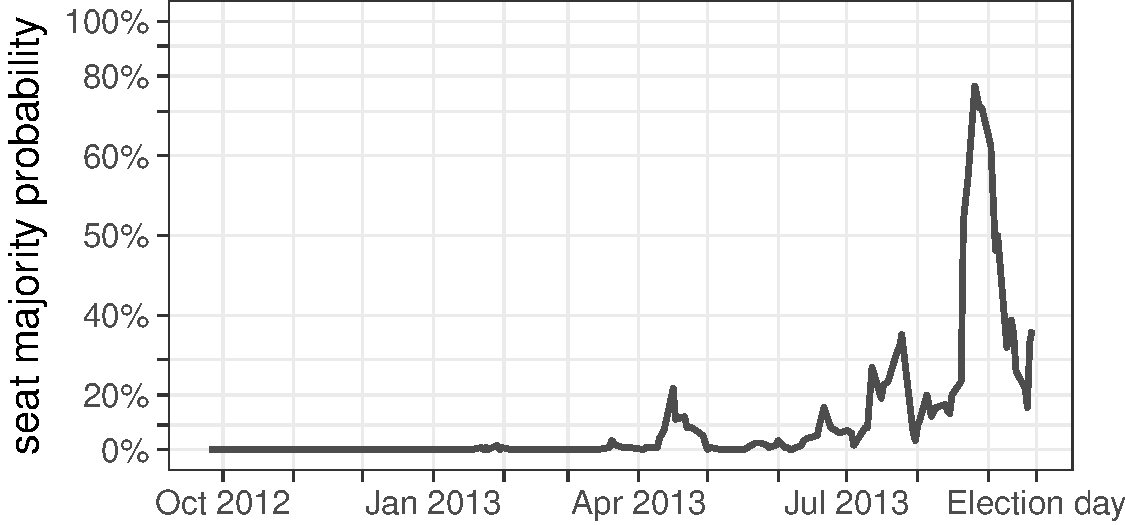
\includegraphics[height=.15\textwidth]{figures/2013_pooled_cdufdp_prob.pdf}
\end{tabular}
\caption{Development of the governing possibility of the coalition Union-FDP before the German federal election in September 2013 based on pooled opinion polls.
Left top: Observed voter shares after redistribution. Left bottom: Probabilities to reach a majority of seats in parliament, based on $10\,000$ simulations. Right: Densities of simulated parliament seat shares based on $10\,000$ simulations. The parts of the densities encoding for seat majorities are colored blue.
\label{fig:2013_cdufdp}
}
\end{figure}

Using the calculated seat majority probabilities together with
the simulated densities instead draws a more comprehensive picture
of the situation. While the overall development of probabilities
growing with time is the same as with the redistributed voter shares,
there are two points that clearly get more weight when shifting 
the focus in reporting from a black-and-white reporting towards
discussing {\it how probable} events are:

First of all, the impact of small changes in voter shares is nicely resembled
in the probability development. Thus, a rise in voter share from $45\%$ to 
$48\%$ in March 2013 only has a very small impact on the absolute
probability, whereas changes near a share of $50\%$ are much more influential.

Second of all, probabilities do not only take the summed party
shares into consideration, but also implicitly cover the 
uncertainty regarding e.g. whether FDP passes the $5\%$ hurdle
or not. Apart from the end of August 2013, FDP passing into the
parliament is highly uncertain and thus majority probabilities for
the coalition are rather small. This can best be seen in the
ridgeline plot (right panel in Fig.~\ref{fig:2013_cdufdp}), where
the densities are bimodal if the raw voter share of FDP is close
to $5\%$ (see Fig.~\ref{fig:2013_fdp}).


\paragraph{FDP passing the 5\% hurdle} \ \\
As mentioned, our approach can also be used to quantify the probability
for other events than seat majorities, e.g. for the FDP successfully
passing the $5\%$ hurdle. Figure~\ref{fig:2013_fdp} again shows that
small changes in raw voter share of the party dramatically influence
the success probabilities. Overall, based on the opinion polls
correctly representing the whole population, a success of the FDP seemed
very uncertain in most times. Only around the end of August 2013
the pooled voter share rose to $6\%$ and the corresponding probability
rose to nearly $100\%$.

\begin{figure}[H]\centering
\begin{tabular}{ll}
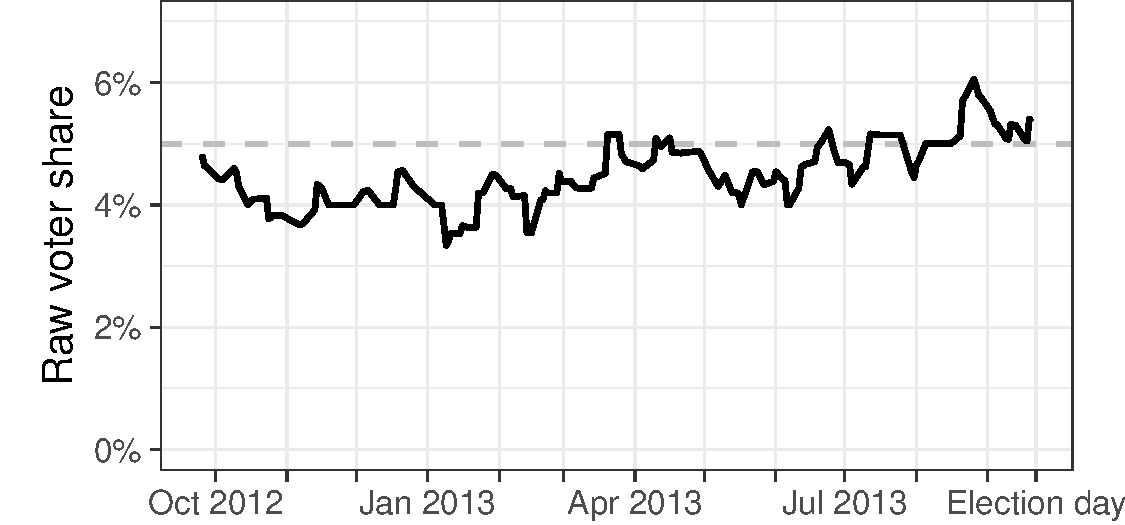
\includegraphics[height=.15\textwidth]{figures/2013_pooled_fdp_rawShares.pdf}
&
\multirow{2}{*}[13ex]{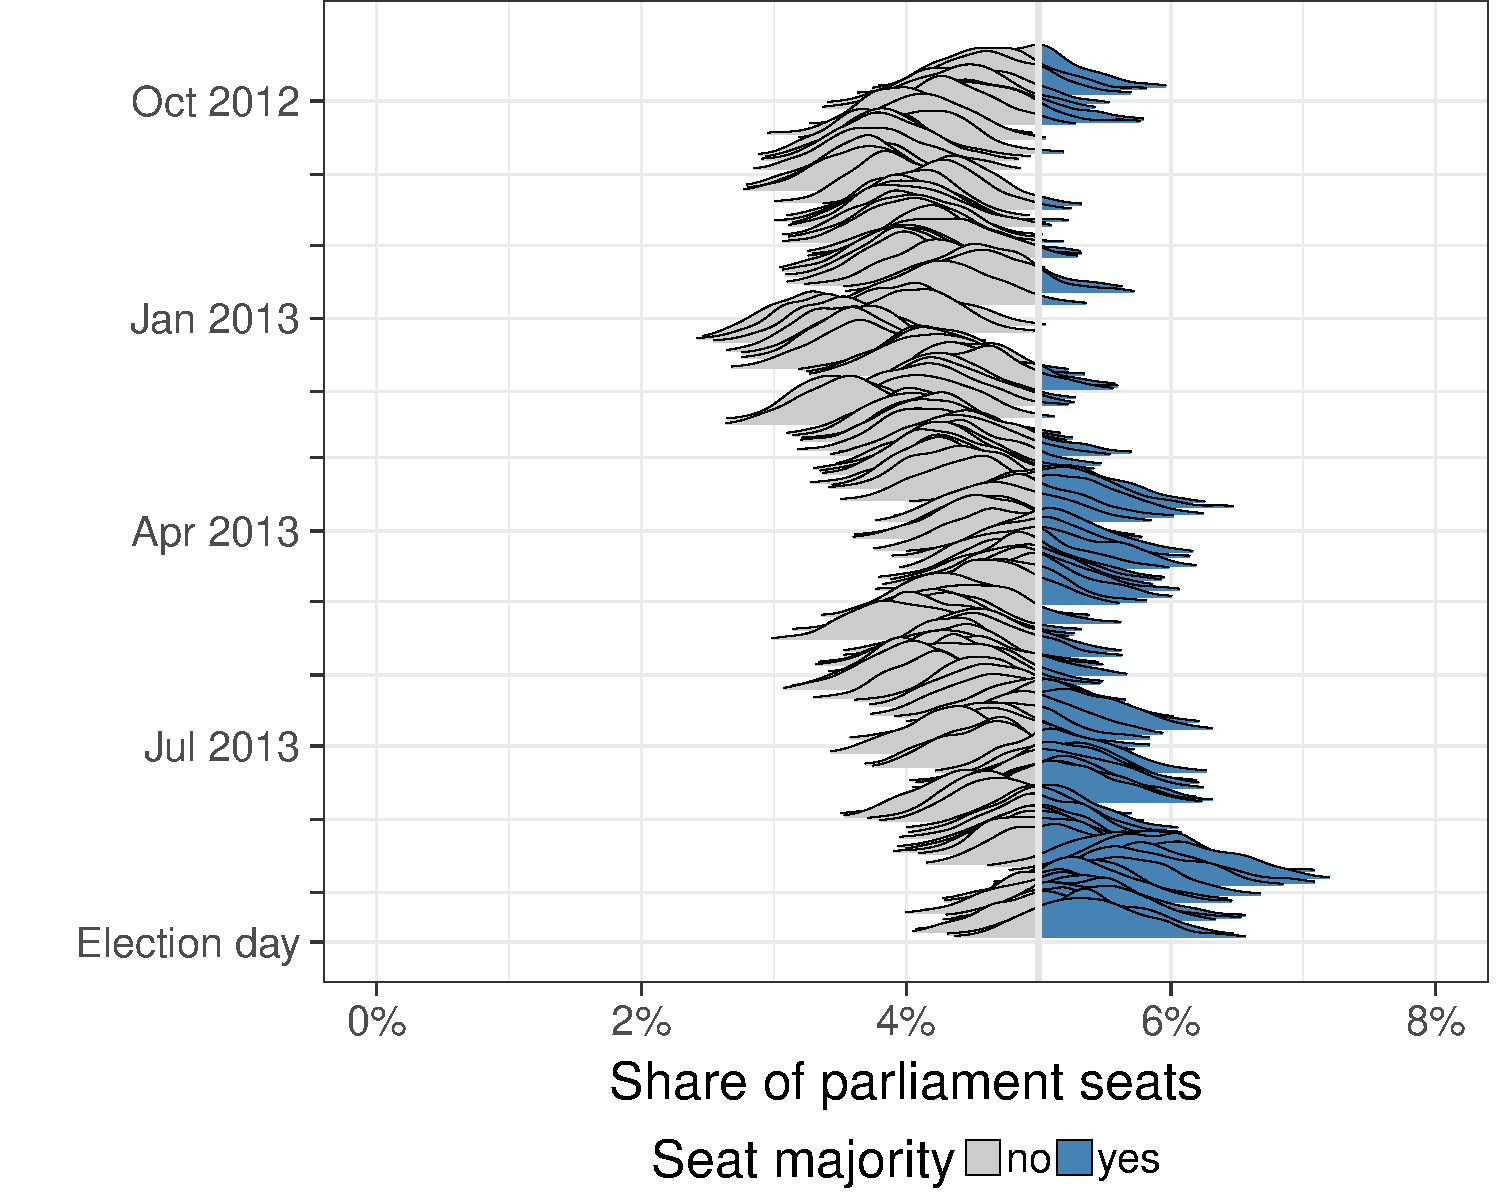
\includegraphics[height=30ex]{figures/2013_pooled_fdp_ridgeline.pdf}}
\\
\includegraphics[height=.15\textwidth]{figures/2013_pooled_fdp_passingProb.pdf}
\end{tabular}
\caption{Development of the chance of FDP to pass the $5\%$ hurdle before the German federal election in September 2013 based on pooled opinion polls.
Left top: Observed voter shares before redistribution. Left bottom: Probabilities to pass the $5\%$ hurdle, based on $10\,000$ simulations. Right: Densities of simulated raw voter shares based on $10\,000$ simulations. The parts of the densities encoding for successfully possing the hurdle are colored blue.
\label{fig:2013_fdp}
}
\end{figure}





\subsection{German federal election 2017} \label{subsec:2017}
Similar to the previous election, prior to the election on
September 24th of 2017 main interest lied in whether Union-FDP
would succeed in getting a seat majority in parliament.
However, the situation differed regarding that the FDP in opinion
polls was safely over $5\%$ (cf. Fig.~\ref{fig:2017_afd}).
The same was true for the right-wing party AfD, which in 2013
slightly failed to getting into parliament. Also, another potential
left-wing coalition between SPD, the green party and the Left
was a valid option to a Union-reigned coalition.


\paragraph{Union-FDP coalition majority} \ \\
The development of redistributed voter shares and majority probabilities
for Union-FDP over the window of one year before election day
is depicted in Figure~\ref{fig:2017_cdufdp}.
Especially as FDP was at all times over $5\%$ in the pooled opinion polls,
the development of voter shares is much more smooth, compared to 
the development of 2013.
Again, it can be seen that even very small changes in voter share
cause immense changes in probability. E.g., at the end of August 2017,
the seat majority probability rises by $30\%$ and reaches its
maximum, only caused by a voter share rise of around $1\%$.
Also, according to the ridgeline plot, redistributed voter shares of under
$47\%$ usually correspond to negligibly small majority probabilities.

\begin{figure}[H]\centering
\begin{tabular}{ll}
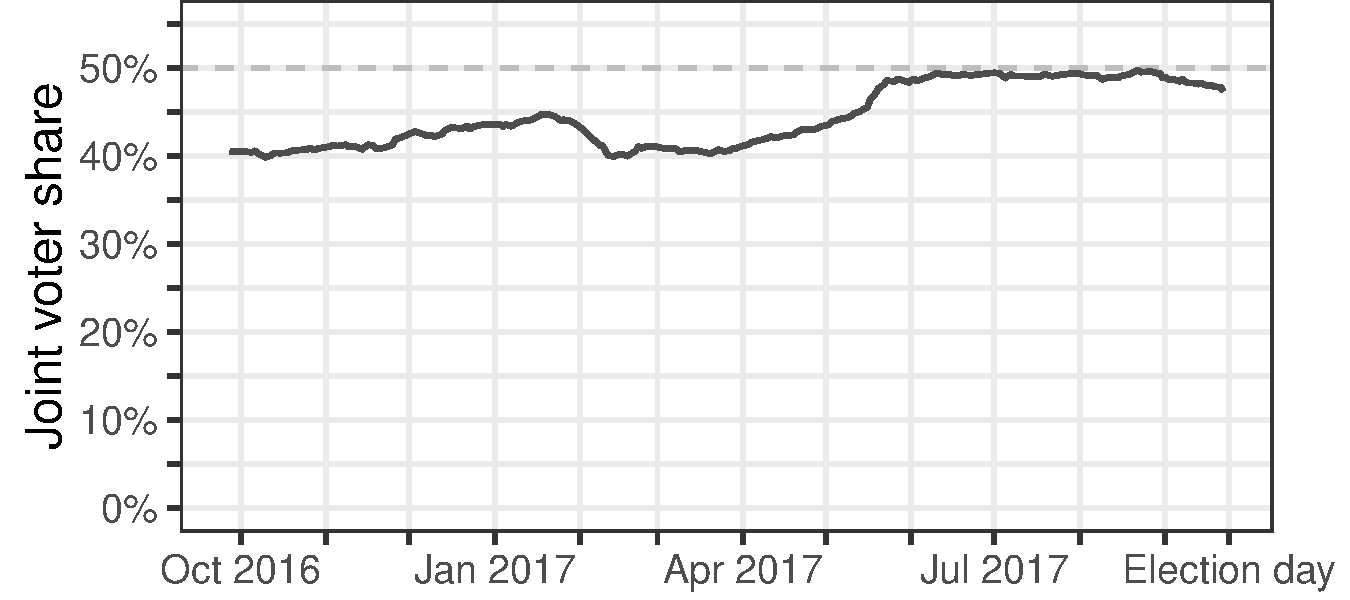
\includegraphics[height=.15\textwidth]{figures/2017_pooled_cdufdp_rawSharesRedist.pdf}
&
\multirow{2}{*}[13ex]{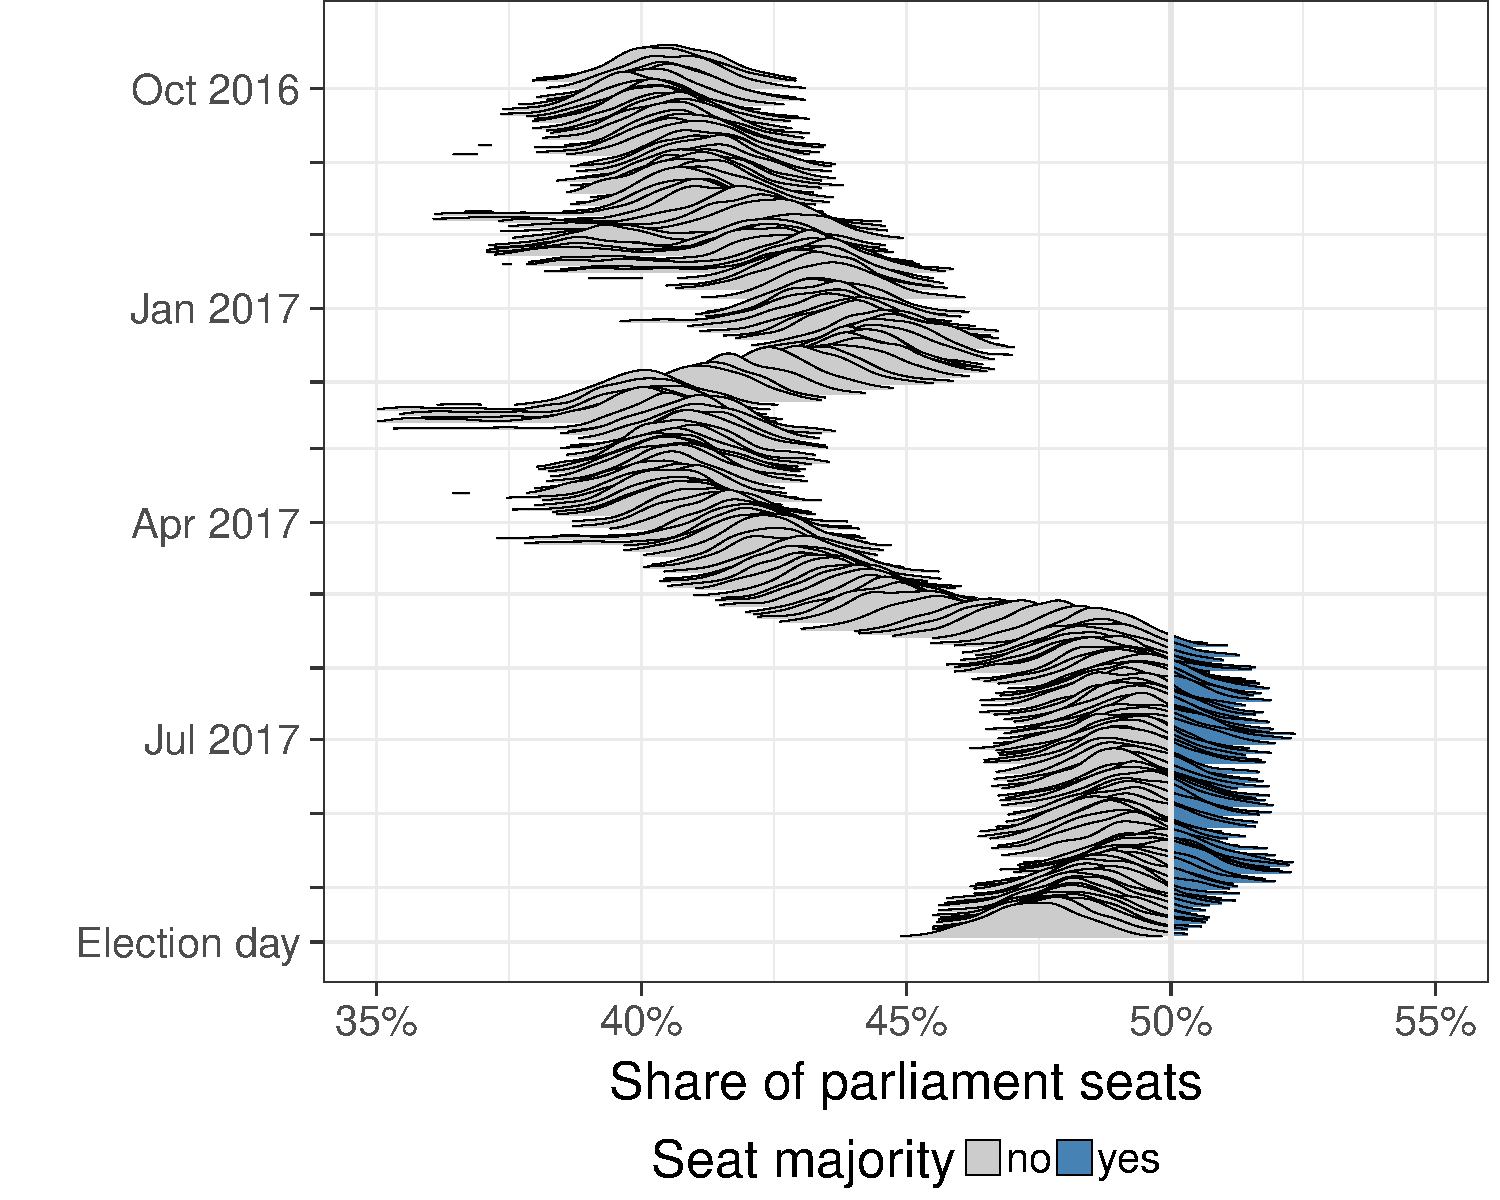
\includegraphics[height=30ex]{figures/2017_pooled_cdufdp_ridgeline.pdf}}
\\
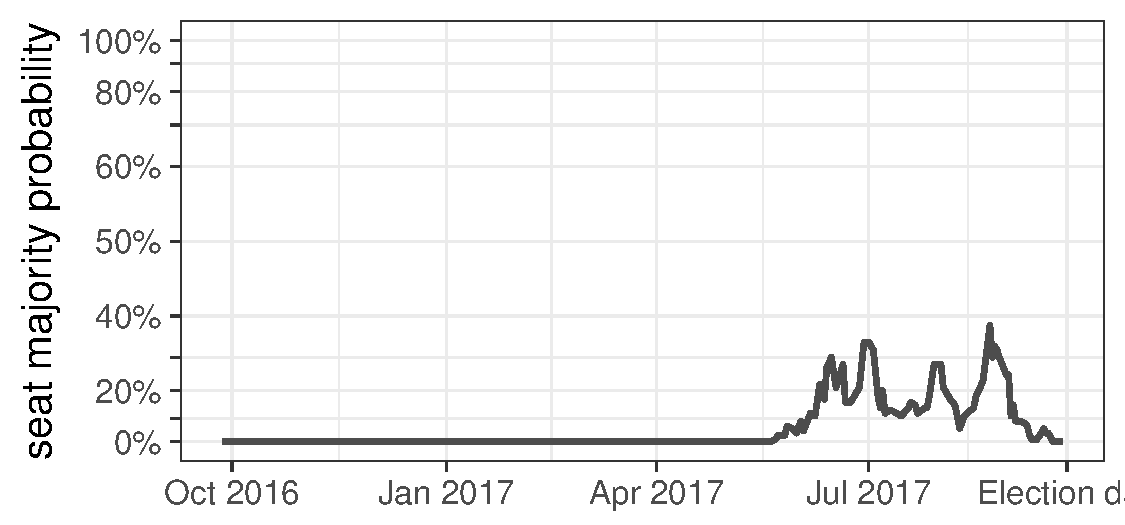
\includegraphics[height=.15\textwidth]{figures/2017_pooled_cdufdp_prob.pdf}
\end{tabular}
\caption{Development of the governing possibility of the coalition Union-FDP before the German federal election in September 2017 based on pooled opinion polls.
Left top: Observed voter shares after redistribution. Left bottom: Probabilities to reach a majority of seats in parliament, based on $10\,000$ simulations. Right: Densities of simulated parliament seat shares based on $10\,000$ simulations. The parts of the densities encoding for seat majorities are colored blue.
\label{fig:2017_cdufdp}
}
\end{figure}


\paragraph{SPD-Left-Greens coalition majority} \ \\
The same as for Union-FDP holds for the potential coalition of
SPD, Greens and Left (see Fig.~\ref{fig:2017_spdleftgreens}).
Between February and April 2017 the redistributed voter
shares reach a high plateau near $50\%$, and there a small change
of about $1\%$ at the end of March 2017 causes a rise of
the probability of over $35\%$.
In the end, especially SPD voter shares declined as heavily as
they rose at the beginning of 2017, and thus a majority of
the coalition shortly before election day was very unlikely.

\begin{figure}[H]\centering
\begin{tabular}{ll}
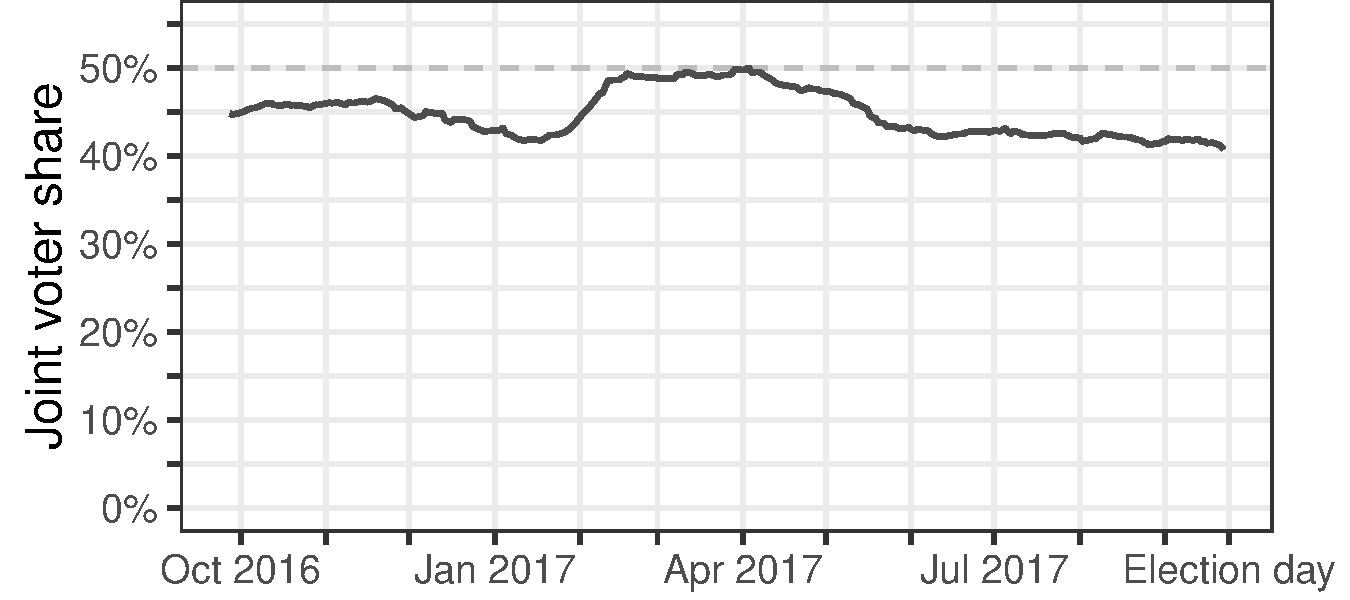
\includegraphics[height=.15\textwidth]{figures/2017_pooled_spdleftgreens_rawSharesRedist.pdf}
&
\multirow{2}{*}[13ex]{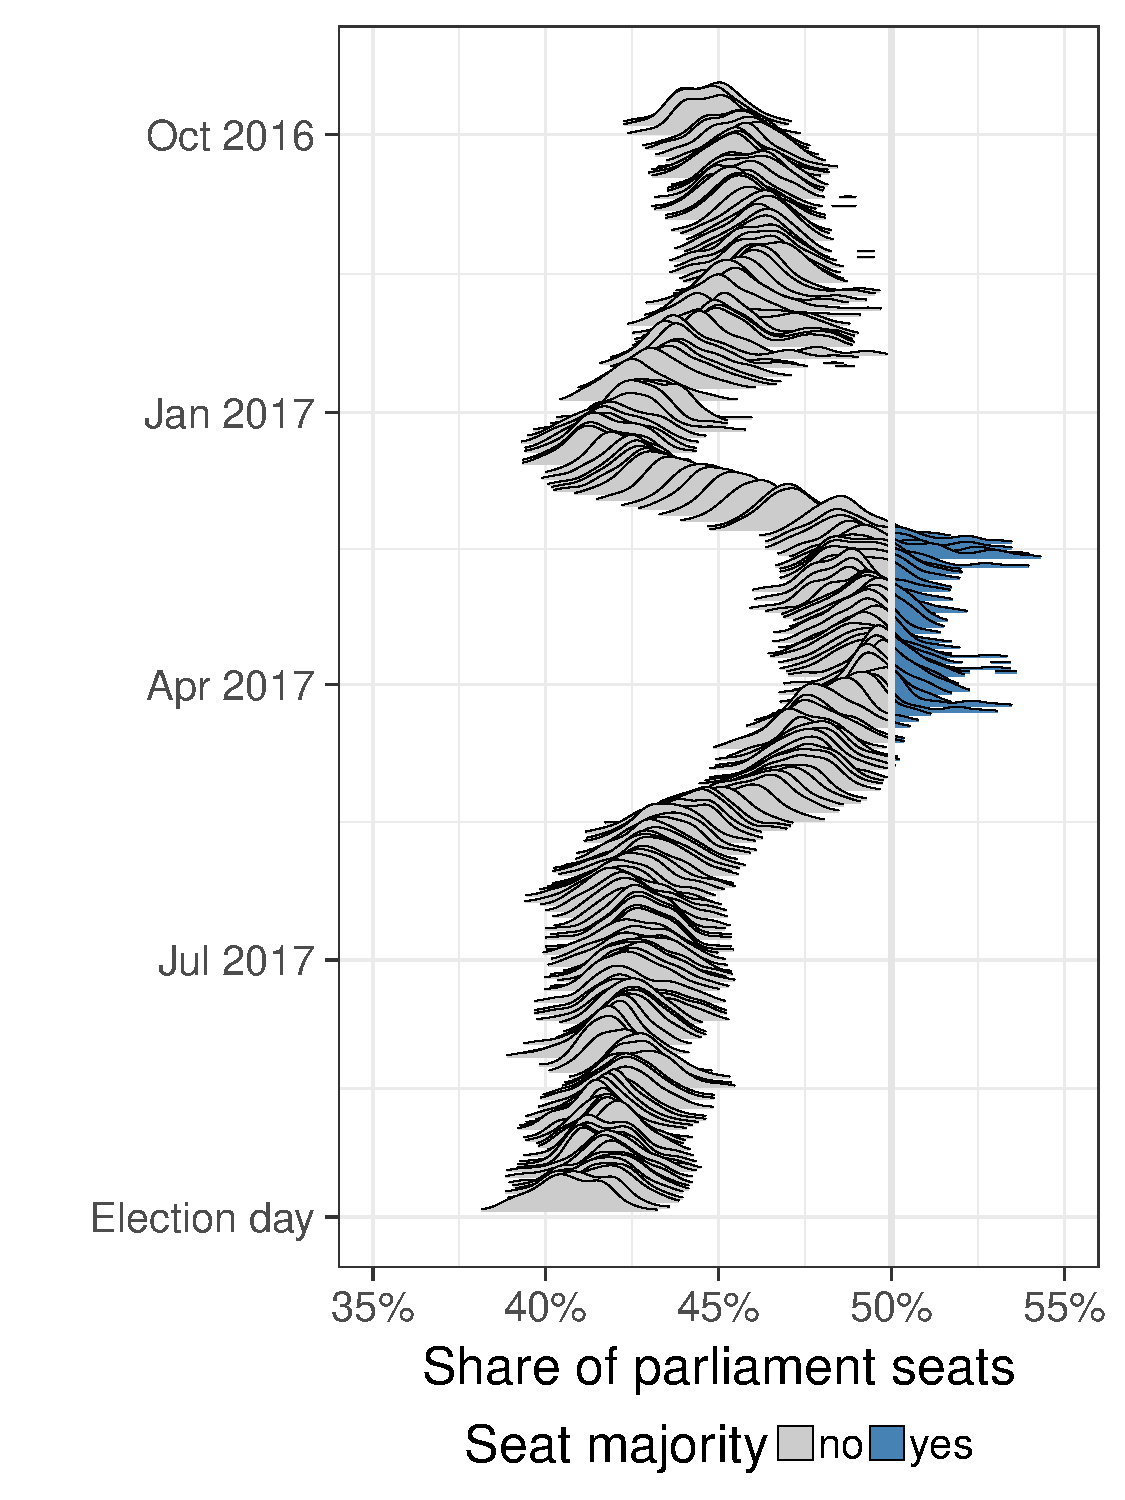
\includegraphics[height=30ex]{figures/2017_pooled_spdleftgreens_ridgeline.pdf}}
\\
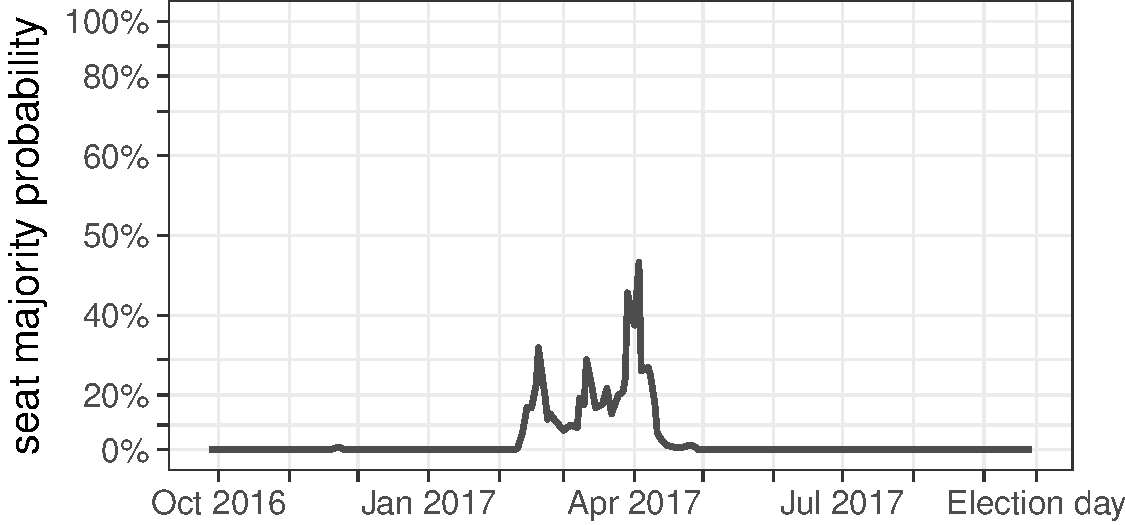
\includegraphics[height=.15\textwidth]{figures/2017_pooled_spdleftgreens_prob.pdf}
\end{tabular}
\caption{Development of the governing possibility of the coalition SPD-Left-Greens before the German federal election in September 2017 based on pooled opinion polls.
Left top: Observed voter shares after redistribution. Left bottom: Probabilities to reach a majority of seats in parliament, based on $10\,000$ simulations. Right: Densities of simulated parliament seat shares based on $10\,000$ simulations. The parts of the densities encoding for seat majorities are colored blue.
\label{fig:2017_spdleftgreens}
}
\end{figure}


\paragraph{AfD becoming third strongest party} \ \\
Specific interest in the election lied in which party would
get the third best result after the major parties Union and SPD.
In the year running up to the election, the right-wing party
AfD oftentimes was leading in raw voter shares (see Fig.~\ref{fig:2017_afd}),
but two weeks before election day three parties were almost
head-to-head.

Using our approach it is easily possible to estimate probabilities
for the event that AfD becomes third biggest party in parliament,
thereby quantifying the sample uncertainty that underlies the
opinion polls and summarizing this complex issue into one
development of probabilities.
The corresponding probability until April 2017
is always at least $70\%$, then varies heavily over the course
of two months, drops to under $10\%$, and rises back up to
over $90\%$ shortly before election day, where the AfD is
nearly $2\%$ over its heaviest competitor -- The Left -- in
absolute raw voter share.

\begin{figure}[H]\centering
\begin{tabular}{l}
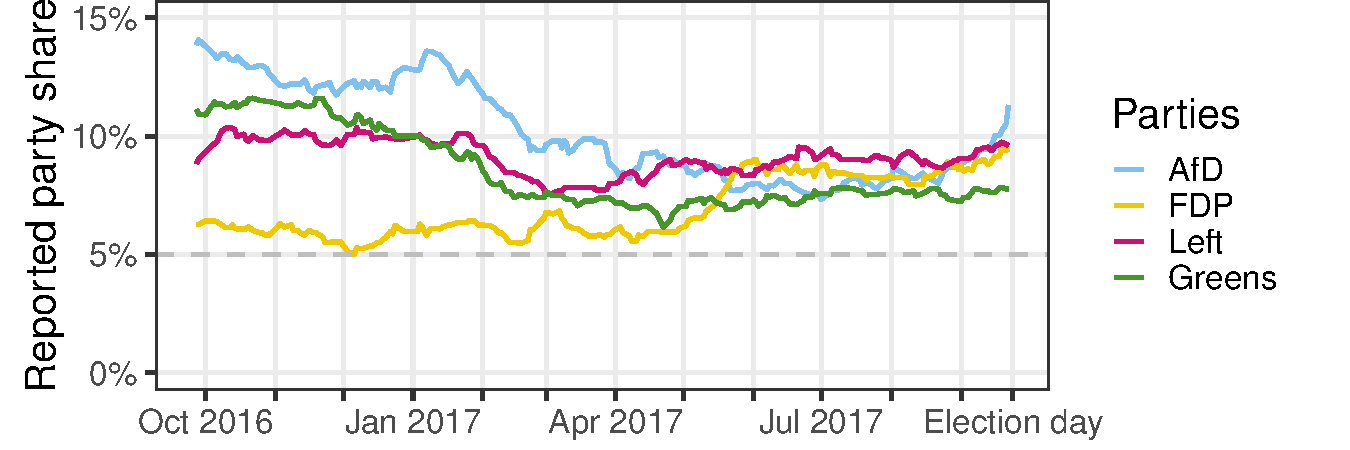
\includegraphics[height=.15\textwidth]{figures/2017_pooled_afd_rawShares.pdf}
\\
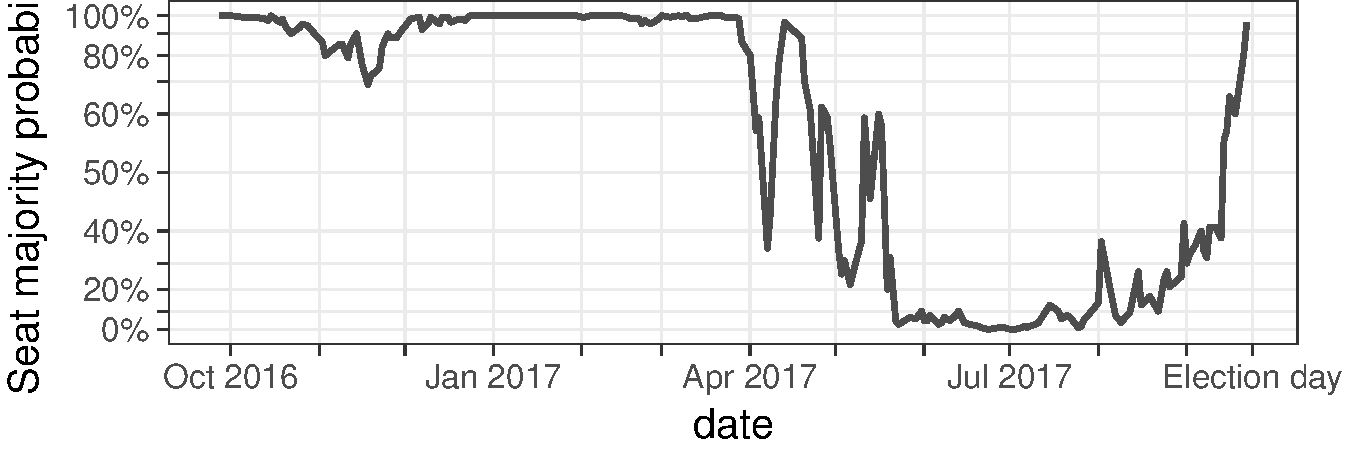
\includegraphics[height=.15\textwidth]{figures/2017_pooled_afd_thirdPartyProb.pdf}
\end{tabular}
\caption{Development of the chance of AfD to become the third strongest party before the German federal election in September 2017 based on pooled opinion polls.
Left top: Observed voter shares before redistribution. Left bottom: Probabilities to become third strongest party, based on $10\,000$ simulations.
\label{fig:2017_afd}
}
\end{figure}

\section{Conclusion} \label{sec:conclusion}
We presented a Bayesian approach to estimate probabilities for specific election outcomes based on
publicly available opinion polls. Pooling allows for the inclusion of information from multiple
surveys and reduces sample uncertainty.
The estimated event probabilities are easy to communicate to the general public and prevent
improper poll-based reporting as they readily include sample uncertainty.
We visualize the results on a publicly available website for chosen elections and
provide the open-source \texttt{R} package \texttt{coalitions} that allows for an easy
application of the method to any multi-party electoral system.
In this manner, our long-term goal is to make proper uncertainty assessment
in general opinion poll-based reporting the rule, rather than an exception.



% % For one-column wide figures use
% \begin{figure}
% % Use the relevant command to insert your figure file.
% % For example, with the graphicx package use
%   \includegraphics{figures/seatDist_ridgeline.pdf}
% % figure caption is below the figure
% \caption{Please write your figure caption here}
% \label{fig:1}       % Give a unique label
% \end{figure}
% %
% % For two-column wide figures use
% \begin{figure*}
% % Use the relevant command to insert your figure file.
% % For example, with the graphicx package use
%   \includegraphics[width=0.75\textwidth]{figures/seatDist_ridgeline.pdf}
% % figure caption is below the figure
% \caption{Please write your figure caption here}
% \label{fig:2}       % Give a unique label
% \end{figure*}
%
% % For tables use
% \begin{table}
% % table caption is above the table
% \caption{Please write your table caption here}
% \label{tab:1}       % Give a unique label
% % For LaTeX tables use
% \begin{tabular}{lll}
% \hline\noalign{\smallskip}
% first & second & third  \\
% \noalign{\smallskip}\hline\noalign{\smallskip}
% number & number & number \\
% number & number & number \\
% \noalign{\smallskip}\hline
% \end{tabular}
% \end{table}


%\begin{acknowledgements}
%If you'd like to thank anyone, place your comments here
%and remove the percent signs.
%\end{acknowledgements}

% BibTeX users please use one of
% \bibliographystyle{spbasic}      % basic style, author-year citations
%\bibliographystyle{spmpsci}      % mathematics and physical sciences
%\bibliographystyle{spphys}       % APS-like style for physics
\bibliography{bauer_2018}   % name your BibTeX data base

% Non-BibTeX users please use
% \begin{thebibliography}{}
%
% and use \bibitem to create references. Consult the Instructions
% for authors for reference list style.
%
% \bibitem{RefJ}
% % Format for Journal Reference
% Author, Article title, Journal, Volume, page numbers (year)
% % Format for books
% \bibitem{RefB}
% Author, Book title, page numbers. Publisher, place (year)
% % etc
% \end{thebibliography}

\end{document}
% end of file template.tex

